\documentclass[11pt,letterpaper]{article}

\usepackage[margin=1in]{geometry}
\usepackage[T1]{fontenc}
\usepackage[utf8]{inputenc}
\usepackage{amsmath}
\usepackage{graphicx}
\usepackage{booktabs}
\usepackage{microtype}
\usepackage{xcolor}
\PassOptionsToPackage{hyphens}{url}
\usepackage[colorlinks=true,linkcolor=blue!50!black,citecolor=blue!50!black,urlcolor=blue!50!black]{hyperref}

\graphicspath{{../figures/}}
\def\UrlBreaks{\do\/\do-\do_\do.\do=}
\Urlmuskip=0mu plus 1mu

% Float placement: keep figures with their text, no float pages holding a single figure
\renewcommand{\topfraction}{0.9}
\renewcommand{\bottomfraction}{0.6}
\renewcommand{\textfraction}{0.07}
\renewcommand{\floatpagefraction}{0.85}

\newcommand{\degC}{$^{\circ}$C}
\newcommand{\Awall}{A_{\mathrm{wall}}/A_{\mathrm{wafer}}}

\title{Every blanket-wafer ALD recipe hides a 40$\times$ under-dose: a chamber-to-feature model of supply-limited atomic layer deposition\thanks{Draft 0.9 (public), 10 November 2026. Every number is from a run documented in the repository run log, \texttt{paper/assumptions.md}.}}

\author{Soham Kavathekar\\[2pt]
\small Department of Chemical and Biomolecular Engineering, University of Pennsylvania,\\
\small Philadelphia, PA 19104, USA\\
\small \href{mailto:sohamuni2024@gmail.com}{sohamuni2024@gmail.com}}

\date{November 2026}

\begin{document}
\maketitle

\begin{abstract}
ALD recipes are tuned on blanket wafers. Product wafers are not blank: a 3D-NAND array of 100\,nm holes at aspect ratio 100 carries 56 times the surface area of the wafer under it, and all of it has to saturate in one pulse. We built a model of a 300\,mm showerhead ALD chamber in which every point on the wafer runs its own feature-scale model of a hole, coupled both ways to the chamber gas, and asked how long the pulse must be. The answer is a single rule: the saturating pulse equals 1.2 times (1 + patterned area ratio) times the time the showerhead needs to deliver one monolayer of precursor. It held within 25\,\% across aspect ratios 20 to 100 and a twenty-fold range of precursor feed; on non-uniform layouts the local wall-area ratio of the densest region sets the pulse, not the wafer average. At a typical operating point the blanket wafer saturates in 0.35\,s and the product wafer in 14\,s. Chamber pressure, showerhead gap and carrier flow do not move that number; precursor delivery rate does. The water half-cycle, fifty times less reactive, needs the same pulse on the product wafer and coats it more evenly. The feature model agrees with an independent Argonne code to 7\,\% and fits published thickness profiles from lateral test structures, and the rule itself reproduces the measured saturation time of a fluidized-bed ALD run on 940\,m$^2$ of silica gel to 7\,\%. The rule turns a day of recipe transfer into arithmetic, and says where a tool's throughput actually comes from.
\end{abstract}

\begin{center}
\fbox{\begin{minipage}{0.94\linewidth}
\vspace{4pt}
\textbf{What this means for a tool (one paragraph for the process engineer).}
If your recipe was saturated on a monitor wafer, multiply the pulse by one plus the product wafer's wall-area ratio before you trust it on product. Size the pulse on the densest or deepest region's own wall-area ratio; the wafer average under-doses it. Pressure, gap and carrier flow are uniformity knobs; they buy no time. Time comes from precursor molecules per second: vapour pressure, bubbler flow, injector design, or an architecture that exposes the wafer to a denser zone (spatial ALD wins by the same factor the rule predicts). Low-sticking reactants are not the bottleneck on patterned wafers; their cost is on blanket wafers only. And when the deepest feature saturates, the chamber shows it: the precursor stops being consumed and appears downstream.
\vspace{4pt}
\end{minipage}}
\end{center}

\section{Introduction}

Three facts set up the problem. First, 3D NAND and DRAM are built from features with aspect ratios of 50 to 100, and ALD is the only way to coat their insides \cite{amat_olympia,amat_centris}, so the precursor must reach the bottom of every feature on the wafer inside a single pulse. Second, the patterned surface area of such a wafer is tens of times the wafer area, so the wafer consumes precursor tens of times faster than the blank wafer the recipe was developed on. Third, nobody models these two things together: feature-scale conformality models \cite{gordon2003,yanguasgil2012,ylilammi2018,cremers2019} assume the precursor density at the feature mouth is given, and chamber models assume the wafer's uptake is given. The quantity that matters, the gas density at the wafer surface while the wafer is eating it, falls between the two.

This paper closes that gap with a model small enough to run on a laptop and checked hard enough to trust. A chamber flow model carries, on every wafer face, a feature-scale model of a hole; the two exchange precursor every time step. The feature model is verified against an independent ballistic code and fitted to published measurements. The result is not a simulation to be rerun for every recipe but a rule: pulse time is set by precursor supply and patterned area, and by nothing else that a chamber recipe normally adjusts.

Equipment makers are building exactly this class of model under the name of equipment-and-process digital twins \cite{amat_blog}. This work is an open, reproducible instance for ALD, with every case file, boundary condition and figure in the repository.

Contributions: (i) a two-way coupled chamber--feature wall condition for OpenFOAM, released; (ii) two-code verification and public-data validation of the feature model; (iii) the supply-limit rule and its range of validity; (iv) the blanket-to-product recipe-transfer factor, the shielding mechanism and the edge-lag inversion; (v) the temporal-versus-spatial design chart and the plasma-ALD recombination ceiling.

\section{Model}

\subsection{Chamber}
Axisymmetric showerhead chamber, 300\,mm wafer, 15\,mm gap, 200\,mm chamber radius, annular outlet. N$_2$ carrier at 300\,Pa, 573\,K ($\rho = 1.76\times10^{-3}$\,kg/m$^3$, $\nu = 1.65\times10^{-2}$\,m$^2$/s), 300\,sccm (0.050\,m/s at the showerhead face), $\mathrm{Re} = 0.045$, residence time 0.53\,s. Steady laminar flow (\texttt{simpleFoam}, OpenFOAM v2606 \cite{openfoam}), frozen for the species step. TMA as a passive scalar $c/c_0$, $D = 8.4\times10^{-3}$\,m$^2$/s at 300\,Pa (Chapman--Enskog scaling), gap P\'eclet number 0.09. Inlet: Danckwerts total-flux condition
\begin{equation}
U\,(c_{\mathrm{face}} - c_0) = D\,\frac{c_{\mathrm{face}} - c_{\mathrm{cell}}}{\delta}.
\end{equation}
We show that a fixed-concentration inlet over-injects by 11$\times$ at this P\'eclet number (Section~\ref{sec:blanket}).

\subsection{Wafer boundary condition (concurrent multiscale)}
Flat surface: irreversible Langmuir,
\begin{equation}
\frac{d\theta}{dt} = \frac{\bar{v}}{4}\, s\,(1-\theta)\,\frac{c_s}{N_0}.
\end{equation}
Holes: cylinder of diameter $d$ and aspect ratio AR, Knudsen diffusivity $d\bar{v}/3$, quasi-steady gas \cite{ylilammi2018} with sink $(\bar{v}/d)\,[\,s\,(1-\theta(x)) + r\,]$, coverage advanced per cell; mouth density equals the local wafer-surface gas density $c_s$. Net uptake per unit wafer area
\begin{equation}
K_{\mathrm{eff}}\, c_s = (1-\phi)\times\text{flat uptake} + \phi\times\text{hole-mouth Knudsen flux},
\end{equation}
$\phi$ the open-area fraction. Implemented as an OpenFOAM mixed condition with value fraction $K_{\mathrm{eff}}/(K_{\mathrm{eff}} + D/\delta)$. Parameters: $s = 5\times10^{-3}$ (TMA) and $10^{-4}$ (H$_2$O) \cite{arts2019jvsta}, $N_0 = 4\times10^{18}$\,m$^{-2}$, $\bar{v}$ from kinetic theory at 573\,K, $d = 100$\,nm, hole density $1.78\times10^{13}$\,m$^{-2}$ (180\,nm hexagonal pitch, 50\,\% of the wafer patterned): open area 14\,\%, $\Awall = 11$, 28, 56 for AR 20, 50, 100.

\subsection{Verification and validation}
\label{sec:vv}
\begin{itemize}
\item Scaling tests on the feature solver: penetration depth $\sim \sqrt{\text{dose}}$; dose for 95\,\% step coverage $\sim \mathrm{AR}^2$ in the diffusion-limited regime (ratio 4.0 for AR 20 $\to$ 40 at $s = 0.5$; drops to 3.2 at $s = 0.05$ where the front becomes reaction-limited); sticking coefficient recovered from a synthetic profile within 5\,\% (log).
\item Two-code check: Machball \cite{machball} (ballistic, cosine re-emission) vs this Knudsen-continuum solver, 95\,\% bottom coverage time at 0.3\,Pa TMA, 573\,K: 1.20 vs 1.29\,s (AR 20), 4.45 vs 4.46\,s (AR 50), 16.2 vs 15.6\,s (AR 100).
\item Embedded-BC check: with negligible hole density the boundary condition's hole-bottom coverage matches the standalone solver driven by the same surface density to 1\,\% at all times.
\item Validation against the Zenodo 3974438 PillarHall Al$_2$O$_3$ profiles \cite{zenodo3974438,yim2020} (TMA/H$_2$O, 300\,\degC, 500 cycles $\times$ 0.1\,s, 500\,nm lateral channel, eight profiles averaged): the slit model with channel narrowing fits the saturation front to an rms of 0.038 of the plateau with $s_{\mathrm{TMA}} = 8.5\times10^{-3}$ (profile-to-profile factor 1.5) and a mouth exposure of 7.5\,Pa\,s per pulse (75\,Pa TMA for 0.1\,s), Fig.~\ref{fig:pillarhall}. The front position (AR 215 at half thickness) fixes the exposure; its width fixes $s$. Published values: 0.5--2$\times10^{-3}$ \cite{arts2019jvsta} (275\,\degC\ set-point); our value is higher, with temperature, the site-density assumption and lumped-vs-explicit kinetics as candidate reasons; $s = 10^{-3}$ at the same exposure is visibly excluded by the data. The chamber runs use $5\times10^{-3}$; the patterned-wafer conclusions are supply-limited and insensitive to it.
\end{itemize}

\begin{figure}[tbp]
\centering
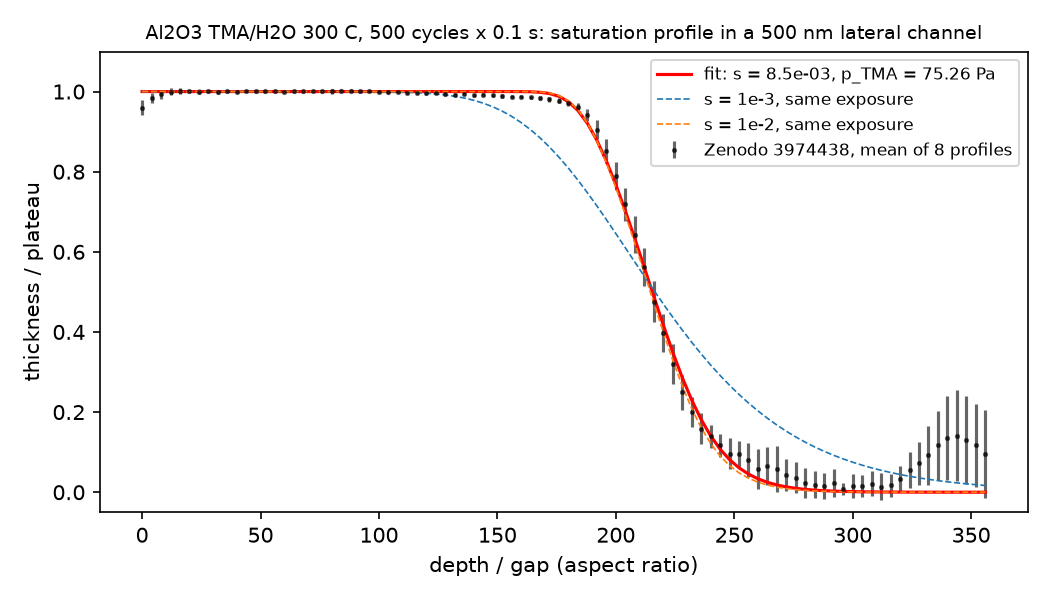
\includegraphics[width=\linewidth]{pillarhall_fit.png}
\caption{Validation of the feature model against the Zenodo 3974438 PillarHall data \cite{zenodo3974438}: the mean of eight measured Al$_2$O$_3$ thickness profiles (TMA/H$_2$O, 300\,\degC, 500 cycles $\times$ 0.1\,s) in a 500\,nm lateral channel, normalised to the plateau thickness and plotted against depth expressed as aspect ratio. The red line is the two-parameter fit of the slit model with channel narrowing ($s_{\mathrm{TMA}} = 8.5\times10^{-3}$, 75\,Pa TMA at the mouth); the dashed lines show $s = 10^{-3}$ and $10^{-2}$ at the same exposure.}
\label{fig:pillarhall}
\end{figure}

\subsection{Validation against a measured high-surface-area ALD run}
\label{sec:powder}
A patterned wafer with tens of wafer-areas of holes is, to the chamber, a powder bed. The cleanest published measurement of supply-limited ALD is Argonne's fluidized-bed Al$_2$O$_3$ run on 940\,m$^2$ of silica gel \cite{lu2022}: in-situ mass spectrometry put TMA breakthrough at 24\,min, and the authors' own accounting gives $0.0115 \pm 0.0020$\,mol of TMA supplied in that time against 0.0103\,mol needed. In the normalisation used throughout this paper, saturation arrived at 1.12 (0.92 to 1.31) times the supply-limit time. Our twelve patterned-wafer cases, with nothing tuned to that experiment, saturate at 1.05 to 1.27 times theirs (Fig.~\ref{fig:validation}); the blanket wafers, at a Damk\"ohler number of 10 instead of hundreds, sit at 1.5 to 4.3 and are the kinetics-limited exception. Argonne's plug-flow theory \cite{lu2022,yanguasgil2024} predicts the same approach to unity from above. A second measured set, TMA utilization in a rotary-drum reactor at five silica-gel loadings from 40 to 1500\,m$^2$ \cite[Table~2]{coile2020}, rises from 25\,\% to 71\,\% with area, i.e.\ saturation moves from 4.0 to 1.4 supply-limit times as the reactor fills with surface; our blanket and patterned wafers (0.07 to 4\,m$^2$) and the fluidized bed (940\,m$^2$, 92\,\%) fall on the same trend across five orders of magnitude of surface area (Fig.~\ref{fig:validation}, right panel).

\begin{figure}[tbp]
\centering
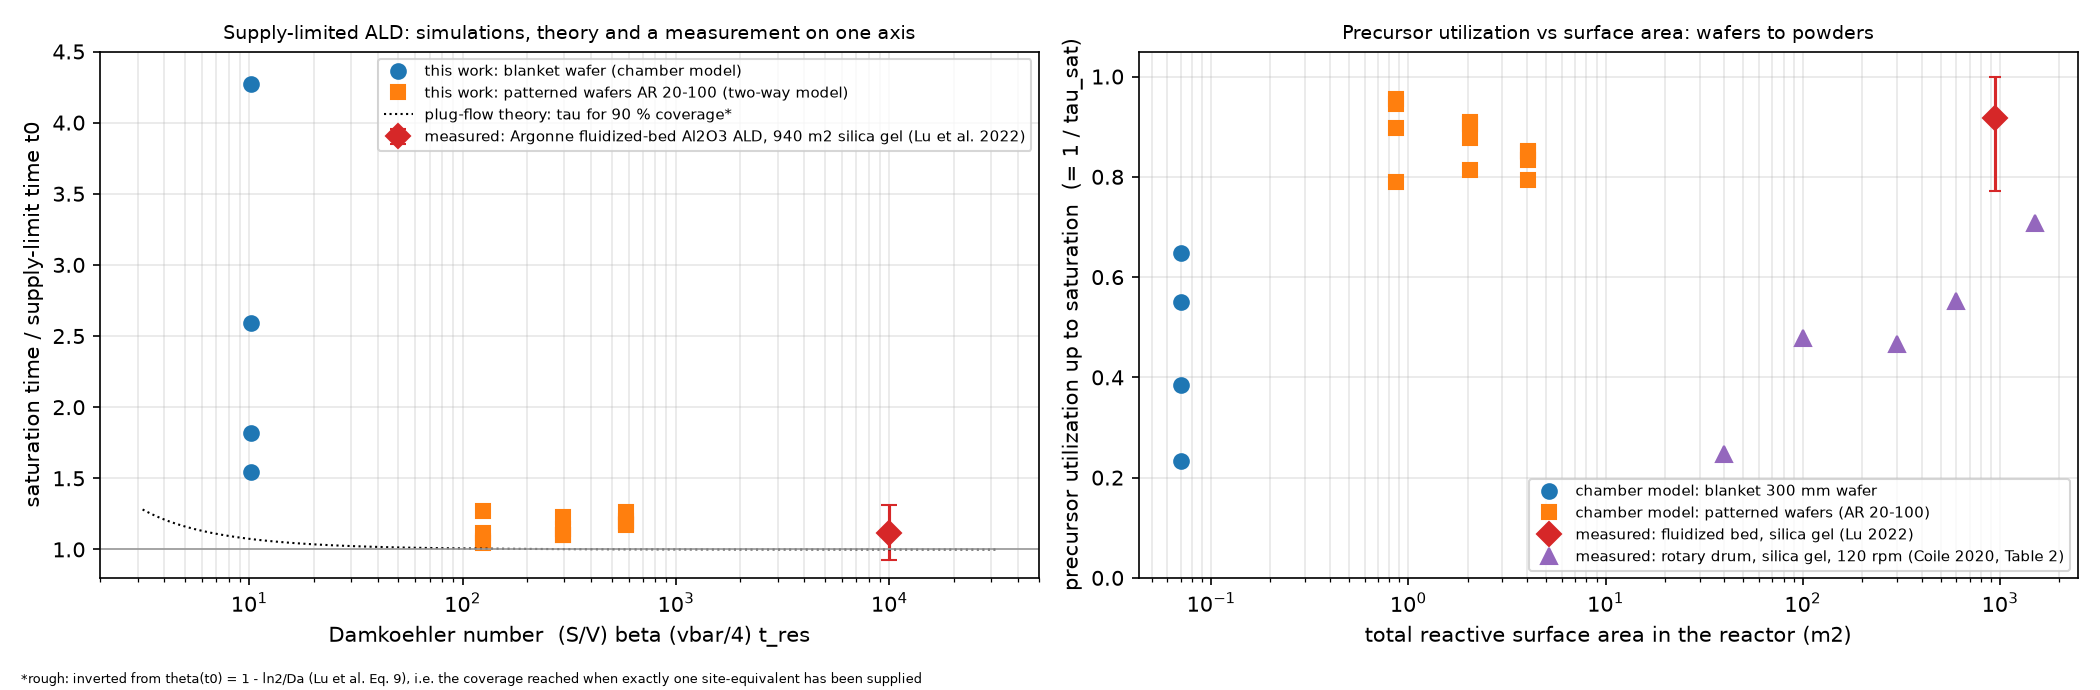
\includegraphics[width=\linewidth]{validation_supply_rule.png}
\caption{The supply-limit rule against measurements. Left: saturation time divided by the supply-limit time $t_0$ versus Damk\"ohler number for the blanket and patterned chamber runs of this work, the plug-flow theory of Lu et al.\ \cite{lu2022}, and the measured Argonne fluidized-bed Al$_2$O$_3$ run on 940\,m$^2$ of silica gel. Right: precursor utilization up to saturation ($= 1/\tau_{\mathrm{sat}}$) versus total reactive surface area in the reactor, from a 0.07\,m$^2$ blanket wafer to 1500\,m$^2$ of powder, with the fluidized-bed point \cite{lu2022} and the rotary-drum loadings of Coile et al.\ \cite{coile2020}.}
\label{fig:validation}
\end{figure}

\section{Results}

\subsection{Blanket wafer}
\label{sec:blanket}
Fixed-concentration inlet absorbs 1179\,\% of the injected TMA; total-flux inlet 96.5\,\%. Centre flux plateaus at the supply rate $U c_0$: at $\mathrm{Pe} = 0.09$ the chamber is supply-limited. Dose uniform to 1\,\% out to $r = 100$\,mm, 7\,\% dip at $r = 142$\,mm (radial sweep), edge spike from the un-patterned floor ring. Gas phase clears 0.05\,s after the pulse. Sticking sweep: capture 96 $\to$ 65\,\%, within-wafer spread 7 $\to$ 0.2\,\%, purge tail 0.15 $\to$ 0.58\,s for $s = 1 \to 10^{-3}$. Self-limiting wafer, $s = 5\times10^{-3}$, 1\,\% TMA: 90\,\% coverage at 0.35\,s (centre), 0.38\,s (edge). Operating sweep: pulse time follows the supply time $N_0/(U c_0)$ at 1.6 to 2.3$\times$; pressure does not change it at fixed sccm but raises the edge lag from 5\,\% (100\,Pa) to 14\,\% (1000\,Pa); a 10\,mm gap beats 25\,mm on time and uniformity.

\subsection{One-way coupling and the shielding effect}
Driving a 100\,nm hole with the blanket wafer's surface density: AR 50 bottom saturates at 0.92\,s, against 4.45\,s at constant density, because the flat surface stops consuming TMA at 0.35\,s and the surface density rises tenfold. AR 100: 3\,\% coverage at the bottom after a 1\,s pulse. Radius shifts the AR 50 time by only 10\,\%.

\subsection{Two-way coupling: loading}
\label{sec:loading}
3D-NAND-like wafer, AR 100, 1\,\% TMA: surface density collapses to $0.019\,c_0$ ($0.24\,c_0$ blanket), the wafer captures 94\,\% of the injected TMA during a 1\,s pulse, and nothing saturates; a 1\,s pulse delivers 8\,\% of the demand. Long pulses (Fig.~\ref{fig:loading}): hole bottoms reach 90\,\% at 14.05\,s (centre), 13.3\,s (edge); flat regions between holes at 1.95\,s (0.35\,s blanket). 3\,\% TMA: 4.75\,s.

\begin{figure}[tbp]
\centering
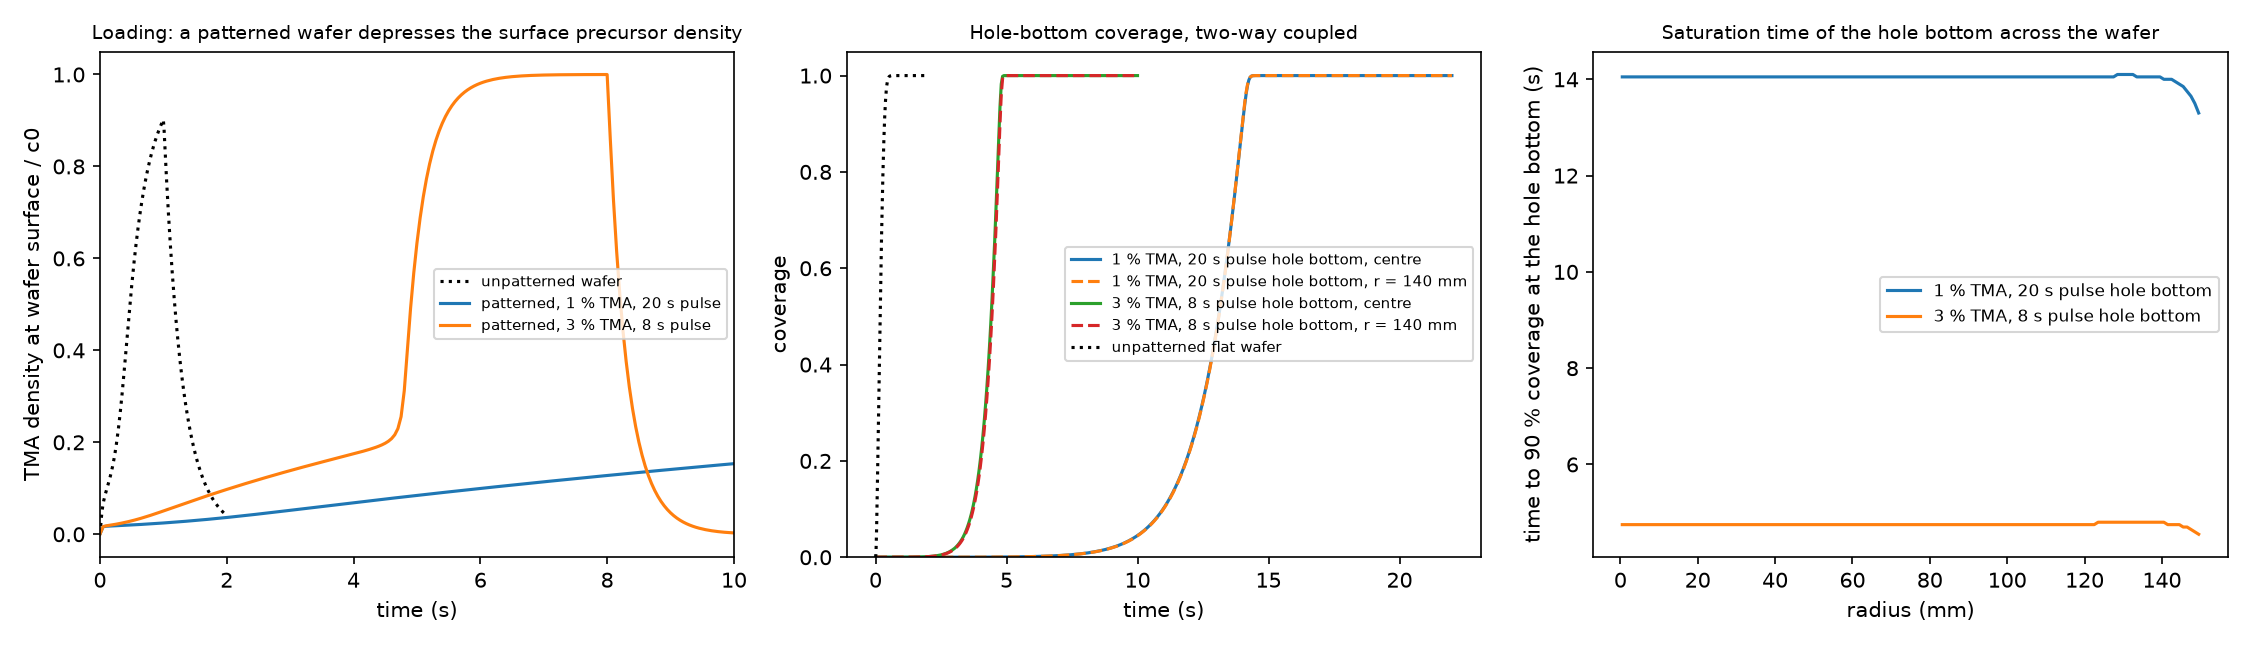
\includegraphics[width=\linewidth]{coupling_patterned_long.png}
\caption{Two-way coupling on the 3D-NAND-like AR-100 wafer, 1\,\% TMA, 300\,sccm, 20\,s pulse. Left: TMA density at the wafer surface relative to $c_0$ for the unpatterned and the patterned wafer, showing the loading effect. Centre: hole-bottom coverage versus time at the wafer centre and at $r = 140$\,mm, with the unpatterned flat wafer for comparison. Right: time to 90\,\% coverage at the hole bottom across the wafer radius.}
\label{fig:loading}
\end{figure}

\subsection{The pulse-time map and the design rule}
\label{sec:rule}
Table~\ref{tab:map} gives the saturating pulse at the worst point on the wafer, and Fig.~\ref{fig:map} plots it. Patterned wafers sit at 1.05 to 1.25$\times$ the supply limit $(1 + \Awall)\,N_0/(U c_0)$ over the whole map; blanket wafers at 1.4 to 3.5$\times$ their own limit, rising with feed fraction as kinetics takes over. Design rule:
\begin{equation}
t_{\mathrm{pulse}} \approx 1.2\,\bigl(1 + \Awall\bigr)\,\frac{N_0}{U c_0}.
\label{eq:rule}
\end{equation}

\begin{table}[tbp]
\centering
\caption{Pulse time to 90\,\% coverage at the worst point on the wafer, from sixteen two-way multiscale runs in the baseline chamber (300\,Pa, 300\,sccm, 15\,mm gap; $s = 5\times10^{-3}$, $N_0 = 4\times10^{18}$\,m$^{-2}$). Patterned wafers carry 100\,nm holes at AR 20, 50 and 100, i.e.\ wall area 11, 28 and 56 times the wafer area.}
\label{tab:map}
\begin{tabular}{lcccc}
\toprule
TMA fraction & Blanket & AR 20 bottoms & AR 50 bottoms & AR 100 bottoms \\
 & (s) & (s) & (s) & (s) \\
\midrule
0.5\,\% & 0.65 & 5.37 & 13.4 & 28.1 \\
1\,\%   & 0.38 & 2.71 & 6.73 & 14.1 \\
3\,\%   & 0.18 & 0.95 & 2.32 & 4.79 \\
10\,\%  & 0.09 & 0.33 & 0.75 & 1.51 \\
\bottomrule
\end{tabular}
\end{table}

\begin{figure}[tbp]
\centering
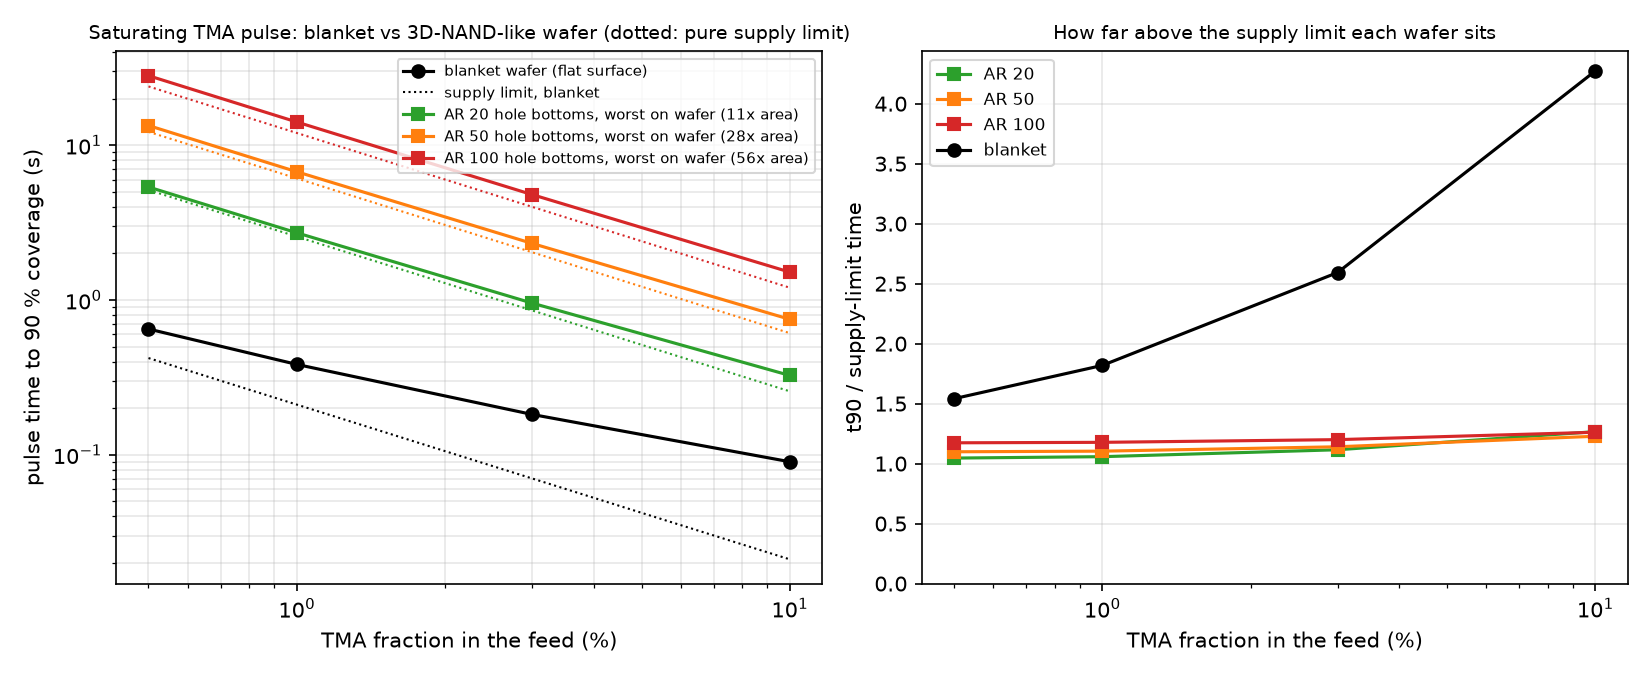
\includegraphics[width=\linewidth]{pulse_time_map.png}
\caption{The pulse-time map. Left: saturating TMA pulse (time to 90\,\% coverage at the worst point on the wafer) versus TMA fraction in the feed for the blanket wafer and for 3D-NAND-like wafers with AR 20, 50 and 100 hole bottoms; the dotted line is the pure supply limit for the blanket wafer. Right: the same times divided by each wafer's own supply-limit time, showing the patterned wafers at 1.05--1.25 and the blanket wafer at 1.4--3.5.}
\label{fig:map}
\end{figure}

\subsection{H$_2$O half-cycle}
\label{sec:h2o}
Blanket: 1.74\,s (5$\times$ TMA; $s\bar{v}/4 = 0.02$\,m/s $< U$). Patterned AR 100: 13.4\,s (TMA 14.05\,s), flat-to-bottom lag 2.6\,s against 12\,s for TMA. Cycle time $\sim$30\,s at 1\,\% precursors vs $\sim$2.5\,s blanket. The effect of reversible water adsorption on coverage and on the purge tail is shown in Fig.~\ref{fig:desorption} and discussed in Section~\ref{sec:discussion}.

\begin{figure}[tbp]
\centering
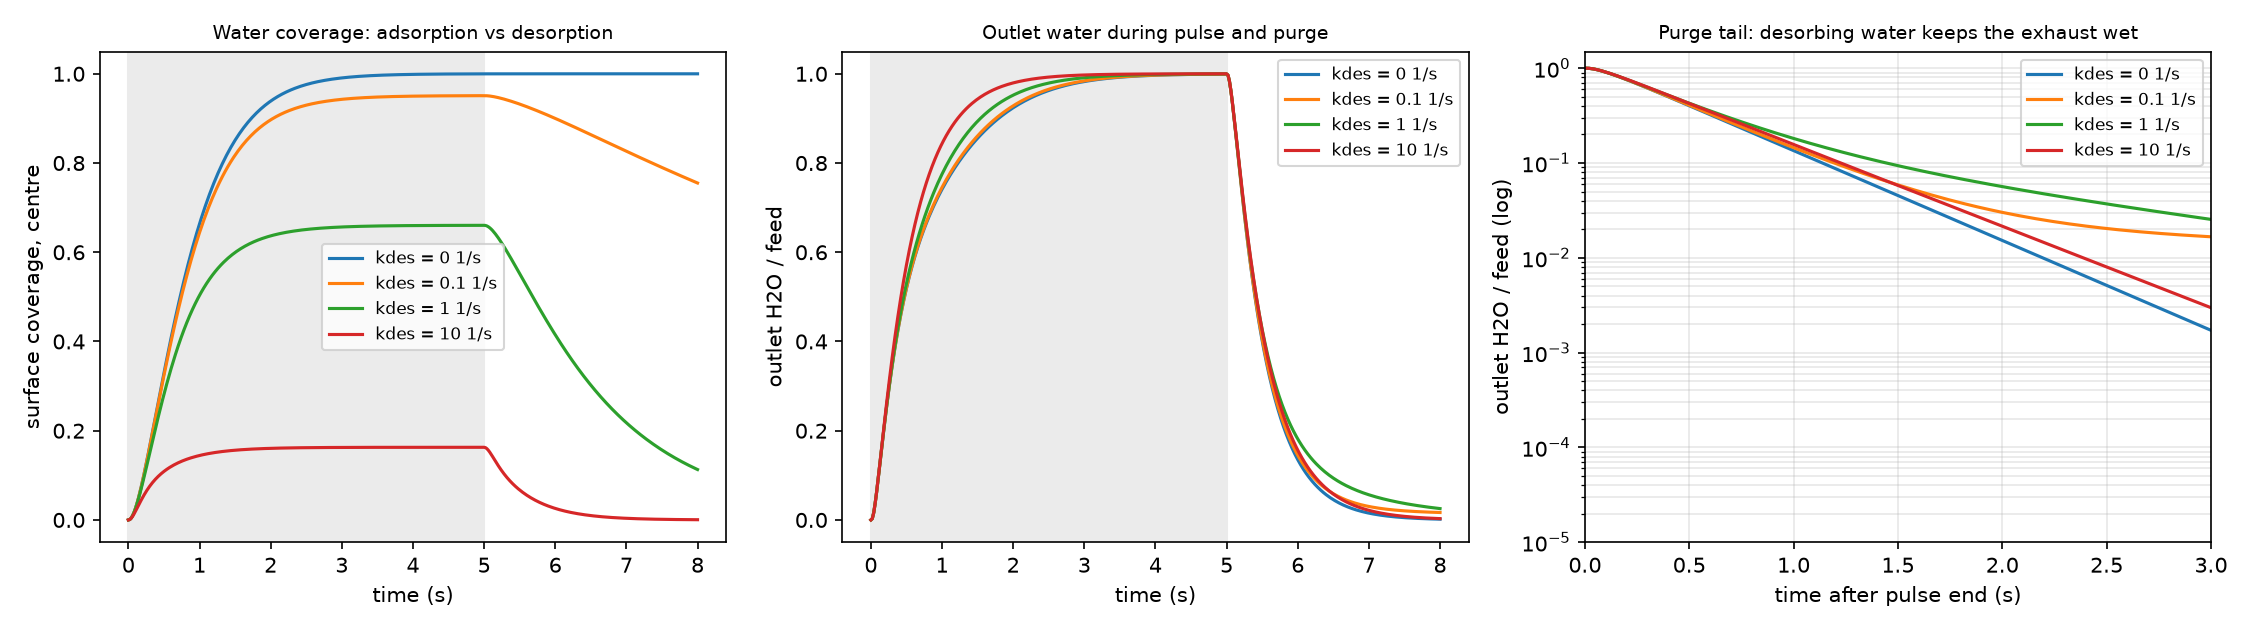
\includegraphics[width=\linewidth]{h2o_desorption.png}
\caption{Reversible water adsorption on the blanket wafer, 1\,\% H$_2$O, 5\,s pulse followed by a 3\,s purge, for first-order desorption rates $k_{\mathrm{des}} = 0$, 0.1, 1 and 10\,s$^{-1}$. Left: surface coverage at the wafer centre. Centre: outlet H$_2$O relative to the feed during pulse and purge. Right: the purge tail on a logarithmic scale; desorbing water keeps the exhaust above 1\,\% of the pulse level for seconds at $k_{\mathrm{des}} = 0.1$ to 1\,s$^{-1}$.}
\label{fig:desorption}
\end{figure}

\subsection{Temporal versus spatial ALD}
\label{sec:spatial}
The design rule gives the molecules required per unit wafer area per half-cycle,
\begin{equation}
\Phi_{\mathrm{req}} = 1.2\,\bigl(1 + \Awall\bigr)\,N_0 .
\end{equation}
A temporal showerhead tool delivers them at $U c_0$ over the whole wafer and pays two purges per cycle; a separated-chemistry (spatial) tool delivers them in passes through a precursor zone at a flux $k$ times the showerhead flux and pays rotation time instead of purges. With $k = 30$, a 1\,s rotation and a 25\,\% zone, the two architectures tie on blanket wafers (2\,s per cycle) and diverge linearly with patterned area: 6.8 vs 2\,s at $\Awall = 11$ (AR 20), 29.9 vs 4\,s at 56 (AR 100), 55.9 vs 8\,s at 112. The crossover lies at $\Awall$ of 5 to 10 for $k = 30$; $k$ is the one quantity a tool maker knows and we do not, so Fig.~\ref{fig:spatial} is a design chart in $k$. This is the quantitative form of the argument behind separated-chemistry ALD architectures for 3D NAND \cite{amat_olympia,amat_patent}.

\begin{figure}[tbp]
\centering
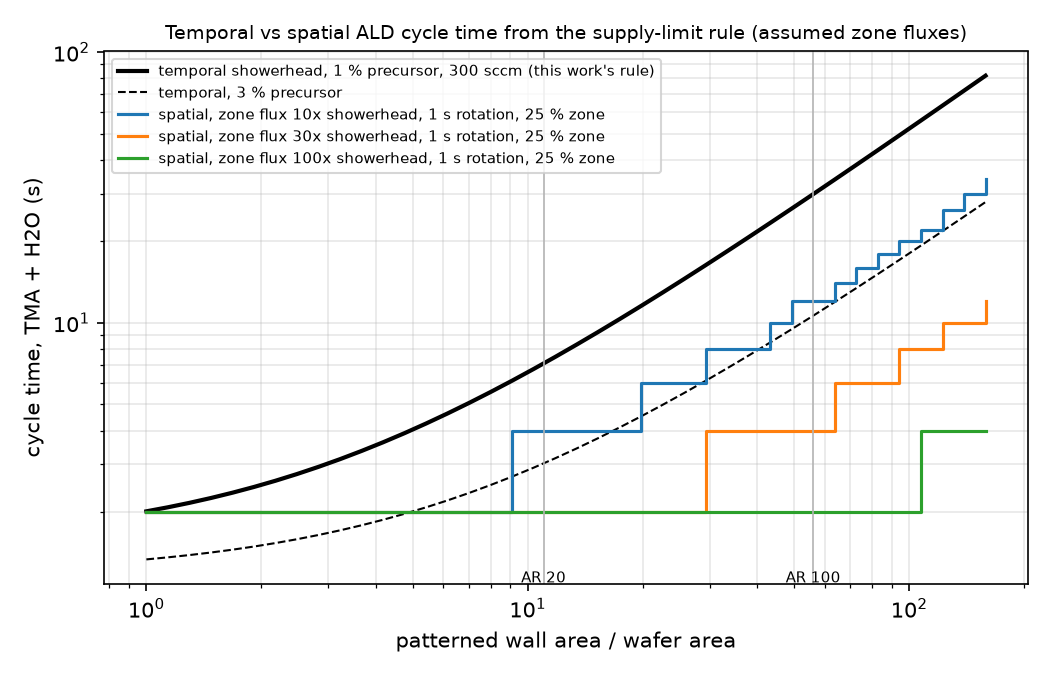
\includegraphics[width=\linewidth]{temporal_vs_spatial.png}
\caption{Temporal versus spatial ALD cycle time (TMA + H$_2$O) from the supply-limit rule, as a function of patterned wall area over wafer area. Solid and dashed black: temporal showerhead tool at 1\,\% and 3\,\% precursor, 300\,sccm, with two purges per cycle. Steps: separated-chemistry (spatial) tool with a precursor-zone flux of 10, 30 and 100 times the showerhead flux, 1\,s rotation and a 25\,\% zone; the zone fluxes are assumed, so the figure is a design chart in $k$. Vertical lines mark AR 20 and AR 100 of the 3D-NAND-like wafer.}
\label{fig:spatial}
\end{figure}

\subsection{Plasma ALD: the recombination ceiling}
\label{sec:peald}
With a wall loss probability $r$ for radicals, the time to 90\,\% bottom coverage in a 100\,nm AR-100 hole rises from 8.0\,s ($r = 0$) to 8.6\,s ($3\times10^{-5}$), 10.2\,s ($10^{-4}$), 16\,s ($3\times10^{-4}$) and 64\,s ($10^{-3}$), and the bottom is not reached at $r \geq 3\times10^{-3}$; the largest aspect ratio saturating within a 5\,s exposure falls from 79 ($r = 10^{-5}$) to 56 ($10^{-3}$) and 29 ($10^{-2}$), Fig.~\ref{fig:peald}. For O atoms on SiO$_2$ and TiO$_2$ ($r \sim 6\times10^{-5}$ \cite{arts2019jpcc,arts2021jpcc}) recombination is a 10 to 25\,\% penalty at AR 100; on high-recombination surfaces it is a hard ceiling that no pulse length removes, and radical flux (plasma source design) or surface chemistry become the levers. The radical sticking coefficient (0.05) is assumed.

\begin{figure}[tbp]
\centering
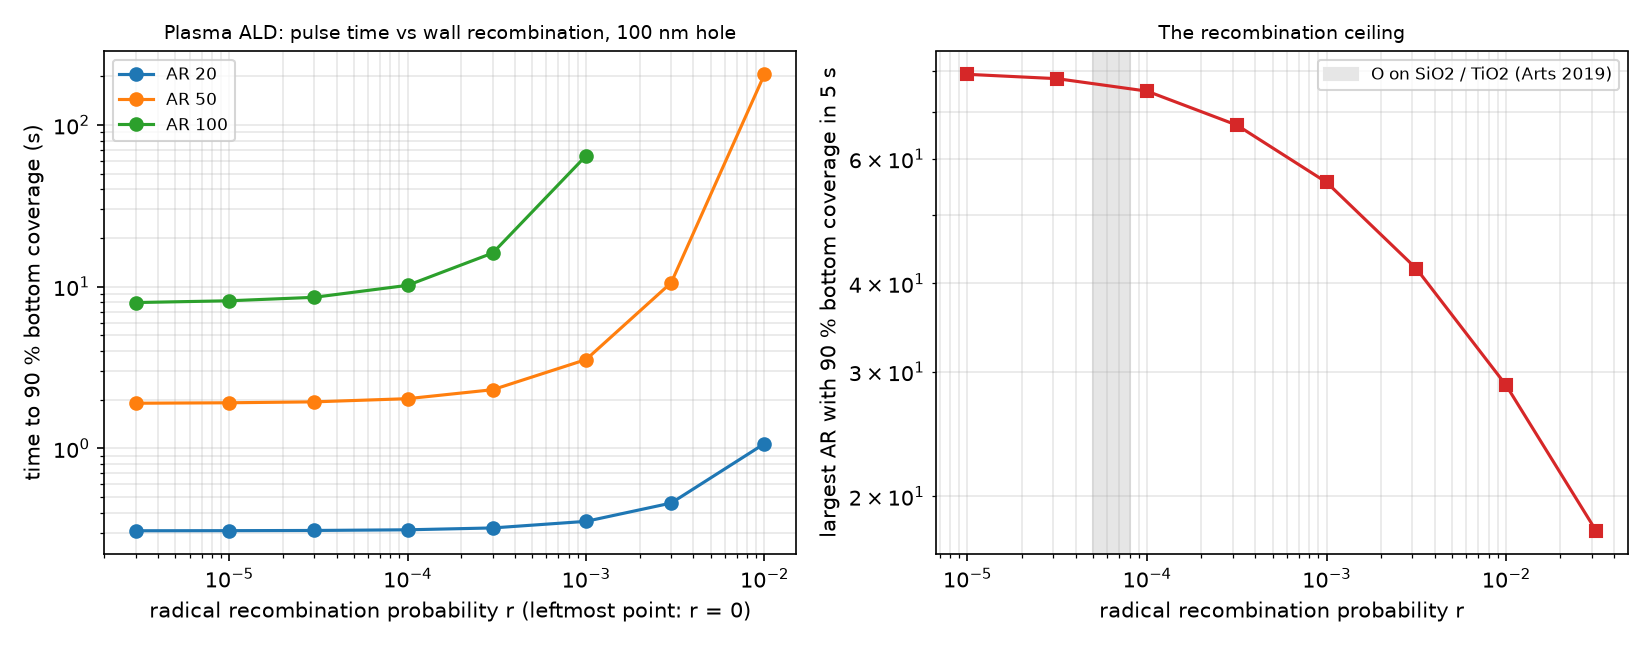
\includegraphics[width=\linewidth]{peald_ceiling.png}
\caption{Plasma ALD in a 100\,nm hole with radical sticking coefficient 0.05. Left: time to 90\,\% bottom coverage versus the radical recombination probability $r$ on the hole walls for AR 20, 50 and 100 (leftmost point: $r = 0$). Right: the largest aspect ratio whose bottom reaches 90\,\% coverage within a 5\,s exposure, versus $r$; the shaded band marks the measured range for O atoms on SiO$_2$ and TiO$_2$ \cite{arts2019jpcc}.}
\label{fig:peald}
\end{figure}

\subsection{Operating optimum and uncertainty}
\label{sec:doe}
A face-centred central composite design (25 two-way runs; TMA fraction 0.5--3\,\%, carrier 150--600\,sccm, pressure 100--1000\,Pa, gap 10--25\,mm) on the AR-100 wafer, fitted as a response surface in JMP and as a Gaussian-process surrogate in MATLAB and scikit-learn (leave-one-out $R^2$ 0.999 for log pulse time, 0.988 for utilization), gives the second-order corrections to the rule (Fig.~\ref{fig:doe}). Pulse time scales as $x^{-1.0}$, $Q^{-0.8}$ and $p^{-0.12}$; the gap is not significant. Precursor utilization up to saturation rises from 68\,\% at 100\,Pa to 88\,\% at 1000\,Pa and falls from 88\,\% at 150\,sccm to 68\,\% at 600\,sccm: carrier gas that is not needed to deliver precursor carries it past the wafer. The fastest point with edge lag under 5\,\% (a constraint never active: lag stays within $-3.5$ to $+1.1$\,\%) is 3\,\%, 600\,sccm, 1000\,Pa, 10\,mm at 2.38\,s. At fixed precursor flow, trading carrier gas for pressure (2.5\,\%, 150\,sccm, 630\,Pa, 10\,mm) cuts the pulse from 11.6 to 9.8\,s and raises utilization from 85 to 94\,\%. A Monte Carlo over the site density (lognormal, factor 1.25) puts a 90\,\% band of 8.2 to 17.2\,s on the 11.9\,s rule prediction at the design centre; the absolute pulse inherits the site-density uncertainty, the ratios in this paper do not. The scikit-learn GP reproduces the MATLAB leave-one-out $R^2$: 0.999 / 0.746 / 0.986 against 0.999 / 0.780 / 0.988 for time / edge lag / utilization. The cost-of-ownership front of pulse time against TMA per saturating pulse, over the factor ranges with edge lag under 5\,\% (Fig.~\ref{fig:pareto}): at the centre point's pulse time (11.6\,s) the front uses 1.044 times the stoichiometric minimum of TMA against 1.181 at the centre, a 12\,\% saving per wafer pass at no cost in time; the last 1\,\% of saving (to 1.030 at 48.9\,s) costs 4.2 times the pulse time.

\begin{figure}[tbp]
\centering
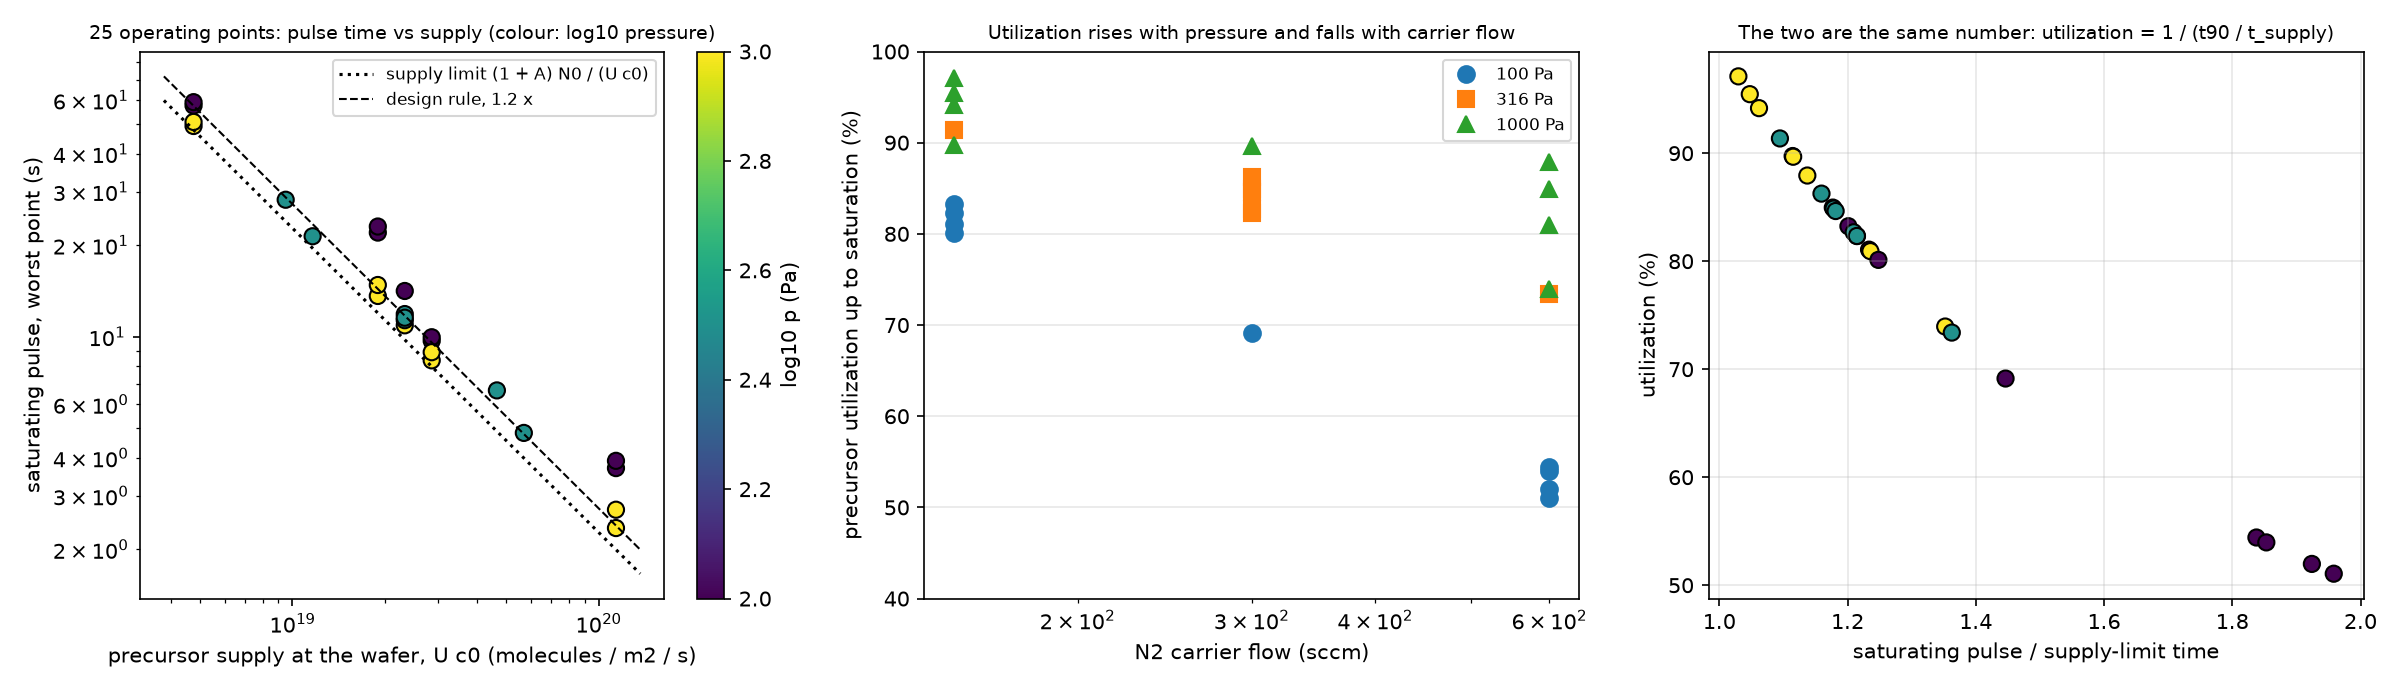
\includegraphics[width=\linewidth]{doe_results.png}
\caption{The 25-run central composite design on the AR-100 wafer. Left: saturating pulse at the worst point on the wafer versus precursor supply at the wafer $U c_0$, coloured by $\log_{10}$ pressure, with the supply limit $(1 + \Awall)\,N_0/(U c_0)$ (dotted) and the 1.2$\times$ design rule (dashed). Centre: precursor utilization up to saturation versus N$_2$ carrier flow at 100, 316 and 1000\,Pa. Right: utilization against the ratio of saturating pulse to supply-limit time, which are the same number.}
\label{fig:doe}
\end{figure}

\begin{figure}[tbp]
\centering
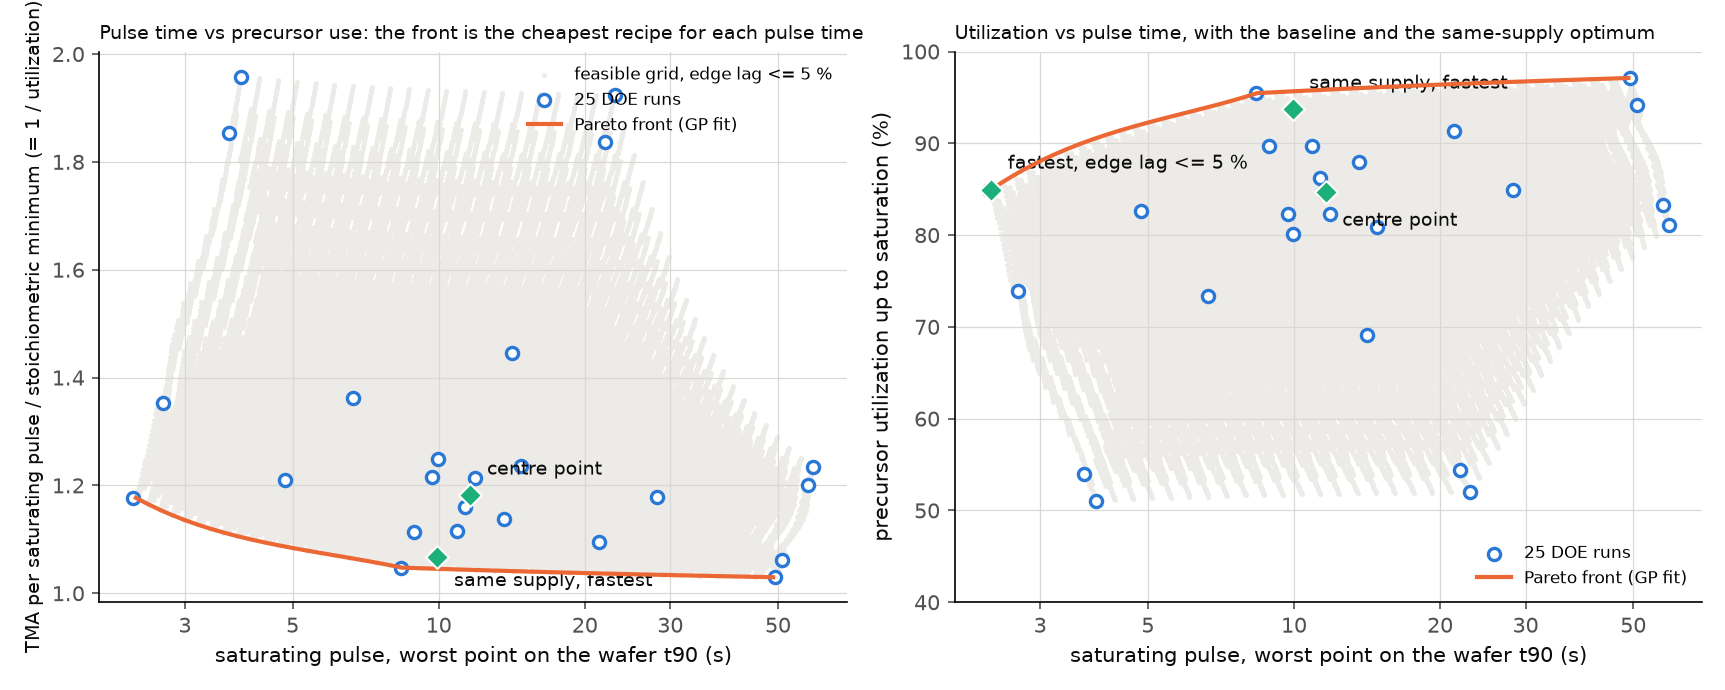
\includegraphics[width=\linewidth]{doe_pareto.png}
\caption{Cost-of-ownership front from the scikit-learn GP surrogate over the DOE factor ranges, restricted to points with edge lag $\leq 5$\,\%. Left: TMA delivered per saturating pulse relative to the stoichiometric minimum ($= 1/\text{utilization}$) versus the saturating pulse at the worst point on the wafer, with the 25 DOE runs, the centre point, the fastest feasible point and the fastest point at the centre's precursor supply. Right: the same front as precursor utilization versus pulse time.}
\label{fig:pareto}
\end{figure}

\subsection{Non-uniform layouts: the local wall-area ratio sets the pulse}
\label{sec:layout}
The patterned-surface boundary condition takes hole density and aspect ratio as functions of radius (\texttt{ARProfile} and \texttt{holeDensityProfile} tables, interpolated at each face; a face with zero hole density is a flat Langmuir surface); the uniform case rerun with the rebuilt library is identical to the original to the 8 written digits at every face and write time. Two layouts at 1\,\% TMA, 300\,sccm, 300\,Pa (Fig.~\ref{fig:layout}): (a) a dense AR-100 centre, full hole density for $r < 75$\,mm ramping to bare wafer at 100\,mm, wafer-average wall-area ratio 19.2; (b) full density everywhere with AR 100 at the centre ramping to 60 at the edge, wafer-average ratio 41.0. The rule with the wafer-average ratio under-predicts both: 5.1\,s against the 11.85\,s the dense centre needs, 10.6\,s against 12.5\,s for the AR ramp. With the local ratio of the most demanding region (55.9 at the centre of both) it predicts 14.4\,s and is conservative by 15 to 21\,\%, against 2\,\% on the uniform wafer; the surplus is what the less-demanding neighbourhood feeds back laterally. A pattern boundary produces a saturation gradient inside the array: 11.85\,s at the centre and 8.75\,s at $r = 74.5$\,mm, the last face at full density, a 26\,\% gradient where the uniform wafer varies by 0.4\,\%. The bare edge of layout (a) saturates 15 to 30\,\% slower than a blanket wafer (flat $t_{90}$ 0.40 to 0.50\,s against 0.35 to 0.38\,s) because the array draws down the gas: surface TMA $0.163\,c_0$ over the bare region at 0.3\,s against $0.24\,c_0$ on a blanket wafer. On the AR ramp the bottom time tracks the local aspect ratio (12.5\,s at AR 100 to 7.6\,s at AR 60) while the flat regions are unaffected (1.95\,s): a 40\,\% depth variation gives a 39\,\% spread in saturation time, so the recipe is set by the deepest tier and shallower regions are over-dosed by their depth ratio.

\begin{figure}[tbp]
\centering
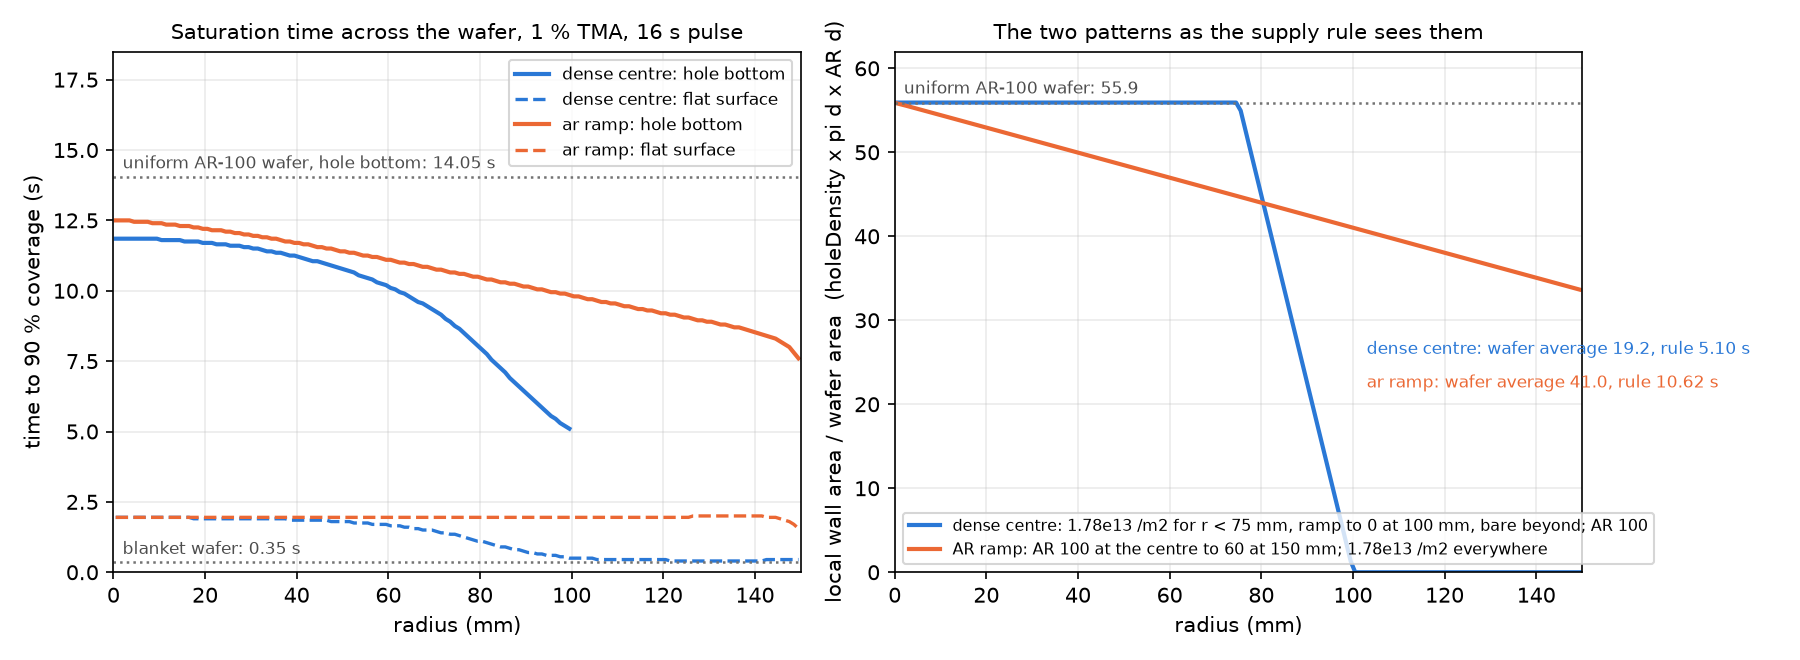
\includegraphics[width=\linewidth]{pattern_layout.png}
\caption{Two non-uniform layouts at 1\,\% TMA, 300\,sccm, 300\,Pa, 16\,s pulse. Left: time to 90\,\% coverage at the hole bottom (solid) and on the flat surface (dashed) across the wafer for the dense-centre layout (AR 100, full hole density for $r < 75$\,mm ramping to bare wafer at 100\,mm) and the AR-ramp layout (full density, AR 100 at the centre to 60 at the edge), with the uniform AR-100 wafer (14.05\,s) and the blanket wafer (0.35\,s) as dotted references. Right: the local wall-area ratio of each layout versus radius, with the wafer averages (19.2 and 41.0) and the pulse the rule predicts from them (5.10 and 10.62\,s).}
\label{fig:layout}
\end{figure}

\section{Discussion}
\label{sec:discussion}
\begin{itemize}
\item Throughput on patterned wafers is bought with precursor delivery rate (vapour pressure, bubbler carrier flow, injector design), not with chamber pressure, gap or carrier flow; those knobs move uniformity.
\item Recipe transfer: the blanket-to-product factor is the wall-area ratio, 11 to 56 here; monitor-wafer recipes under-dose product wafers by that factor at the same supply.
\item Precursor utilization: 60\,\% (TMA) and 50\,\% (H$_2$O) over the saturating pulse on the patterned wafer; the remainder is pumped after saturation. Shorter pulses with feedback (end-point on surface density) would recover it.
\item Low sticking is a conformality asset and a throughput cost only on blanket wafers.
\item Robustness checks: replacing the bare floor by a 25\,mm edge ring with pumping below the wafer plane changes no saturation time by more than one write interval and leaves the within-wafer spread within 3\,\% (blanket 9--11\,\%, patterned 4\,\%), Fig.~\ref{fig:edgering}; the pulse-time results do not depend on the chamber outboard of the wafer at this P\'eclet number.
\item Robustness checks continued: 200, 300 and 400\,\degC\ at fixed sccm and feed fraction give the same pulse times within one write interval (the supply $U c_0$ is temperature-independent; temperature acts through the chemistry, held fixed here); 50, 100 and 200\,nm holes at fixed open area and aspect ratio saturate within 1\,\% of each other, so the wall-area ratio is the rule's only geometric input.
\item Limitations: isothermal gas (temperature enters only through properties); frozen carrier flow; irreversible Langmuir in the main runs; a first-order desorption term was added for water and shows the purge-tail mechanism (desorbing water holds the exhaust above 1\,\% for seconds at $k_{\mathrm{des}} = 0.1$ to 1\,s$^{-1}$) and the equilibrium-coverage limit (above $\sim$0.3\,s$^{-1}$ at 1\,\% H$_2$O the surface never reaches 90\,\%), Fig.~\ref{fig:desorption}, but $k_{\mathrm{des}}$ is a parameter, not a measurement, and a two-site chemisorbed/physisorbed model is the next step; single pattern density (14\,\% open area, half the wafer patterned); Knudsen $D_K = d\bar{v}/3$ without Clausing correction; $s$ and $N_0$ are literature-range inputs (PillarHall fit $8.5\times10^{-3}$; Arts et al.\ \cite{arts2019jvsta} 0.5--2$\times10^{-3}$).
\end{itemize}

\begin{figure}[tbp]
\centering
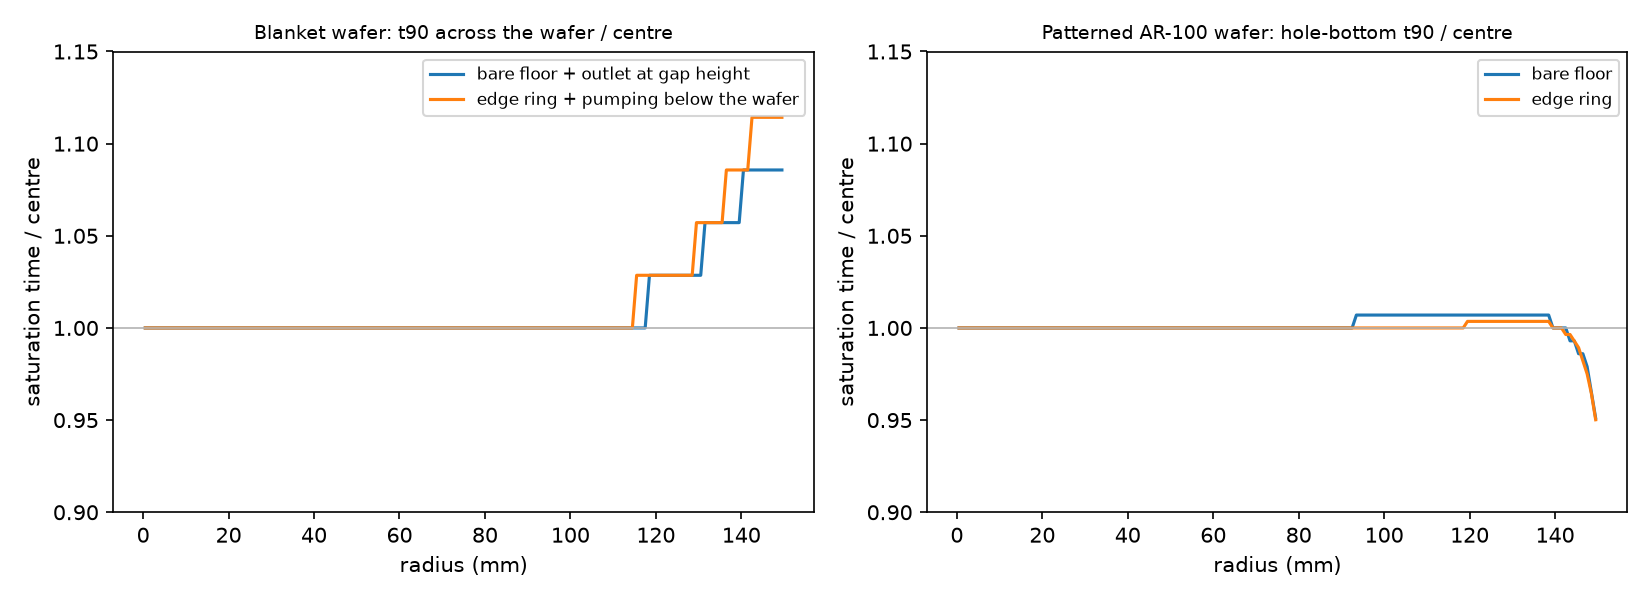
\includegraphics[width=\linewidth]{edgering_comparison.png}
\caption{Robustness to the chamber geometry outboard of the wafer, baseline conditions, 1\,\% TMA. Saturation time across the wafer divided by its value at the centre for the bare floor with the outlet at gap height and for a 25\,mm non-absorbing edge ring with the pumping slot 25\,mm below the wafer plane. Left: blanket wafer. Right: hole-bottom saturation on the patterned AR-100 wafer. The two geometries differ by at most one write interval.}
\label{fig:edgering}
\end{figure}

\section{Conclusions}

\begin{enumerate}
\item On a patterned wafer, the ALD pulse that saturates the deepest feature is set by precursor supply:
\begin{equation}
t_{\mathrm{pulse}} = 1.2\,\bigl(1 + \Awall\bigr)\,\frac{N_0}{U c_0},
\end{equation}
within 25\,\% over aspect ratios 20--100 and a twenty-fold range of feed fraction, and independent of hole diameter at fixed wall area, of temperature at fixed sccm and fraction, and of the chamber geometry outboard of the wafer.
\item The same normalisation puts a measured fluidized-bed ALD run at 1.12 supply-limit times and orders the measured utilization of a rotary-drum reactor with loading; wafers and powders sit on one curve of utilization against surface area spanning five orders of magnitude.
\item A recipe saturated on a blanket wafer under-doses a product wafer by the wall-area ratio, 11 to 56 here. Blanket wafers are the kinetics-limited exception to the rule, not the norm.
\item On a non-uniform layout the pulse is set by the local wall-area ratio of the most demanding region, not by the wafer average: the average under-predicts by 2.3$\times$ (dense centre) and 1.2$\times$ (aspect-ratio ramp), the local ratio is conservative by 15 to 21\,\%, and a pattern boundary puts a 26\,\% saturation gradient inside the array.
\item Second-order knobs: pressure up and carrier flow down raise precursor utilization from about 55\,\% to 95\,\% at fixed precursor flow; gap and pressure set within-wafer edge lag (5 to 18\,\%) but not time.
\item The water half-cycle needs the same pulse as TMA on patterned wafers despite a 50$\times$ lower sticking coefficient, and coats deep features more evenly; reversible adsorption, not chamber flushing, governs its purge.
\item Plasma ALD adds a hard ceiling: above a wall recombination probability of about $3\times10^{-3}$, aspect ratio 100 is unreachable by dose. Separated-chemistry (spatial) architectures beat temporal pulsing by the same wall-area factor the rule predicts.
\item All of this runs on a laptop in open-source tools, with the feature model verified against an independent code and fitted to public measurements, and every number traceable to a script in the repository.
\end{enumerate}

\section*{Acknowledgements}
Validation data by R.~L. Puurunen and O.~M.~E. Ylivaara (Aalto University, Zenodo 3974438, CC BY 4.0). Machball by A.~Yanguas-Gil and J.~W. Elam (Argonne). OpenFOAM v2606 (OpenCFD) via the gerlero/openfoam-app build.

\section*{Code and data availability}
OpenFOAM v2606 cases, the \texttt{aldWallKinetics} boundary-condition library, the Python \texttt{aldconf} solver and its command line (\texttt{python -m aldconf} evaluates the rule, the surrogate and the Pareto front), tests and all figures: \url{https://github.com/Soham-ChemE/ald-conformality}. Validation data: Zenodo 3974438 (CC BY 4.0).

\begingroup
\small
\begin{thebibliography}{99}

\bibitem{gordon2003}
R.~G. Gordon, D.~Hausmann, E.~Kim and J.~Shepard,
``A kinetic model for step coverage by atomic layer deposition in narrow holes or trenches,''
\emph{Chem. Vap. Deposition} \textbf{9}(2), 73--78 (2003).
\href{https://doi.org/10.1002/cvde.200390005}{doi:10.1002/cvde.200390005}.

\bibitem{yanguasgil2012}
A.~Yanguas-Gil and J.~W. Elam,
``Self-limited reaction-diffusion in nanostructured substrates: surface coverage dynamics and analytic approximations to ALD saturation times,''
\emph{Chem. Vap. Deposition} \textbf{18}(1--3), 46--52 (2012).
\href{https://doi.org/10.1002/cvde.201106938}{doi:10.1002/cvde.201106938}.

\bibitem{machball}
A.~Yanguas-Gil and J.~W. Elam,
\emph{Machball: reactive transport inside nanostructured and high-surface-area materials with self-limited surface kinetics}, documentation, Argonne National Laboratory,
\url{https://machball.readthedocs.io/} (accessed November 2026).
The ballistic transport model is described in A.~Yanguas-Gil and J.~W. Elam, ``A Markov chain approach to simulate atomic layer deposition chemistry and transport inside nanostructured substrates,'' \emph{Theor. Chem. Acc.} \textbf{133}, 1465 (2014), \href{https://doi.org/10.1007/s00214-014-1465-x}{doi:10.1007/s00214-014-1465-x}.

\bibitem{ylilammi2018}
M.~Ylilammi, O.~M.~E. Ylivaara and R.~L. Puurunen,
``Modeling growth kinetics of thin films made by atomic layer deposition in lateral high-aspect-ratio structures,''
\emph{J. Appl. Phys.} \textbf{123}, 205301 (2018).
\href{https://doi.org/10.1063/1.5028178}{doi:10.1063/1.5028178}.

\bibitem{arts2019jvsta}
K.~Arts, V.~Vandalon, R.~L. Puurunen, M.~Utriainen, F.~Gao, W.~M.~M. Kessels and H.~C.~M. Knoops,
``Sticking probabilities of H$_2$O and Al(CH$_3$)$_3$ during atomic layer deposition of Al$_2$O$_3$ extracted from their impact on film conformality,''
\emph{J. Vac. Sci. Technol. A} \textbf{37}, 030908 (2019).
\href{https://doi.org/10.1116/1.5093620}{doi:10.1116/1.5093620}.

\bibitem{arts2019jpcc}
K.~Arts, M.~Utriainen, R.~L. Puurunen, W.~M.~M. Kessels and H.~C.~M. Knoops,
``Film conformality and extracted recombination probabilities of O atoms during plasma-assisted atomic layer deposition of SiO$_2$, TiO$_2$, Al$_2$O$_3$, and HfO$_2$,''
\emph{J. Phys. Chem. C} \textbf{123}(44), 27030--27035 (2019).
\href{https://doi.org/10.1021/acs.jpcc.9b08176}{doi:10.1021/acs.jpcc.9b08176}.

\bibitem{arts2021jpcc}
K.~Arts, S.~Deijkers, R.~L. Puurunen, W.~M.~M. Kessels and H.~C.~M. Knoops,
``Oxygen recombination probability data for plasma-assisted atomic layer deposition of SiO$_2$ and TiO$_2$,''
\emph{J. Phys. Chem. C} \textbf{125}(15), 8244--8252 (2021).
\href{https://doi.org/10.1021/acs.jpcc.1c01505}{doi:10.1021/acs.jpcc.1c01505}.

\bibitem{cremers2019}
V.~Cremers, R.~L. Puurunen and J.~Dendooven,
``Conformality in atomic layer deposition: current status overview of analysis and modelling,''
\emph{Appl. Phys. Rev.} \textbf{6}, 021302 (2019).
\href{https://doi.org/10.1063/1.5060967}{doi:10.1063/1.5060967}.

\bibitem{yim2020}
J.~Yim, O.~M.~E. Ylivaara, M.~Ylilammi, V.~Korpelainen, E.~Haimi, E.~Verkama, M.~Utriainen and R.~L. Puurunen,
``Saturation profile based conformality analysis for atomic layer deposition: aluminum oxide in lateral high-aspect-ratio channels,''
\emph{Phys. Chem. Chem. Phys.} \textbf{22}(40), 23107--23120 (2020).
\href{https://doi.org/10.1039/D0CP03358H}{doi:10.1039/D0CP03358H}.

\bibitem{zenodo3974438}
J.~Marles, O.~M.~E. Ylivaara and R.~L. Puurunen,
``ALD Al$_2$O$_3$ thickness profile in microscopic rectangular channel: TMA/H$_2$O, 300\,\degC, 500 cycles, PillarHall LHAR3 (500\,nm gap),'' dataset, Zenodo, version 1.0.0 (2021), CC BY 4.0.
\href{https://doi.org/10.5281/zenodo.3974438}{doi:10.5281/zenodo.3974438}.

\bibitem{jarvilehto2023}
J.~J\"arvilehto, J.~A. Velasco, J.~Yim, C.~Gonsalves and R.~L. Puurunen,
``Simulation of conformality of ALD growth inside lateral channels: comparison between a diffusion--reaction model and a ballistic transport--reaction model,''
\emph{Phys. Chem. Chem. Phys.} \textbf{25}(34), 22952--22964 (2023).
\href{https://doi.org/10.1039/D3CP01829F}{doi:10.1039/D3CP01829F}.

\bibitem{lu2022}
Z.~Lu, A.~Yanguas-Gil, D.~Kang, P.~Darapaneni, A.~U. Mane, C.~L. Marshall and J.~W. Elam,
``Scalable synthesis of supported catalysts using fluidized bed atomic layer deposition,''
\emph{J. Vac. Sci. Technol. A} \textbf{40}(4), 042404 (2022).
\href{https://doi.org/10.1116/6.0001891}{doi:10.1116/6.0001891}; OSTI 1902316.

\bibitem{yanguasgil2024}
A.~Yanguas-Gil and J.~W. Elam,
``Modeling scale-up of particle coating by atomic layer deposition,''
arXiv:2408.13116 (2024).
\href{https://doi.org/10.48550/arXiv.2408.13116}{doi:10.48550/arXiv.2408.13116}.

\bibitem{coile2020}
M.~W. Coile, M.~J. Young, J.~A. Libera, A.~U. Mane and J.~W. Elam,
``High-capacity rotary drum for atomic layer deposition onto powders and small mechanical parts in a hot-walled viscous flow reactor,''
\emph{J. Vac. Sci. Technol. A} \textbf{38}(5), 052403 (2020).
\href{https://doi.org/10.1116/6.0000274}{doi:10.1116/6.0000274}; OSTI 1660751.

\bibitem{amat_blog}
U.~Kelkar, ``Semiconductor equipment and processes need digital twins,'' Applied Materials blog, 5 July 2023.
\url{https://www.appliedmaterials.com/us/en/blog/blog-posts/semiconductor-equipment-and-processes-need-digital-twins.html} (accessed November 2026).

\bibitem{amat_olympia}
Applied Materials, Inc., ``Applied Materials introduces high-performance ALD technology for the 3D era,'' press release (Applied Olympia ALD system), Santa Clara, CA, 13 July 2015.
\url{https://ir.appliedmaterials.com/news-releases/news-release-details/applied-materials-introduces-high-performance-ald-technology-3d} (accessed November 2026).

\bibitem{amat_centris}
Applied Materials, Inc., ``Applied Materials unveils deposition and selective etch systems to advance 3D chip scaling,'' press release (Centris Spectral SiN ALD system), 15 June 2026.
\url{https://www.appliedmaterials.com/us/en/newsroom/press-releases/061526-applied-materials-unveils-deposition-selective-etch-systems-to-advance-3d-chip-scaling.html} (accessed November 2026).

\bibitem{amat_patent}
N.~Li, V.~Nguyen, M.~Balseanu, L.-Q. Xia, S.~D. Marcus, H.~Yang and K.~Tanaka (Applied Materials, Inc.),
``Seamless gap-fill with spatial atomic layer deposition,'' US patent application publication US\,2015/0255324\,A1, published 10 September 2015.

\bibitem{openfoam}
OpenCFD Ltd., \emph{OpenFOAM v2606}, June 2026, \url{https://www.openfoam.com}; built for macOS with the gerlero/openfoam-app distribution, \url{https://github.com/gerlero/openfoam-app} (accessed November 2026).

\end{thebibliography}
\endgroup

\end{document}
